\chapter{Implementation}

%The implementation should look at any issues you encountered as you tried to implement your design. During the work, you might have found that elements of your design were unnecessary or overly complex; perhaps third party libraries were available that simplified some of the functions that you intended to implement. If things were easier in some areas, then how did you adapt your project to take account of your findings?

%It is more likely that things were more complex than you first thought. In particular, were there any problems or difficulties that you found during implementation that you had to address? Did such problems simply delay you or were they more significant?

%You can conclude this section by reviewing the end of the implementation stage against the planned requirements.

\section{Image processing}
The image processing would prove to be an integral part of the application, enhancing the ability to learn handwriting more effectively and efficiently. The end script was implemented over a series of sprints.
\subsection{Optimising Tesseract}
After the design considerations to use OpenCV was chosen, specific algorithms would need to be implemented. After a discussion with Dr Hannah Dee, it was suggested that investigations into different binarisation scripts would be useful.

\subsubsection{OTSU}
[CITE CITE, Lab brooks page]

OTSU, created by Nobuyuki Otsu, is a binarisation technique which essentially converts an image to black and white. Otsu is a global thresholding algorithm, using the whole image as a comparsion. This is unlike local thresholding algorithms where comparisons are made pixel by pixel.CITE Automatic thresholding for defect detection].

Due to notes having non-uniform lighting by the intrusion of shadows on an image, this makes OTSU difficult to reliably binarise the image.

\begin{figure}[H]
  \centering
  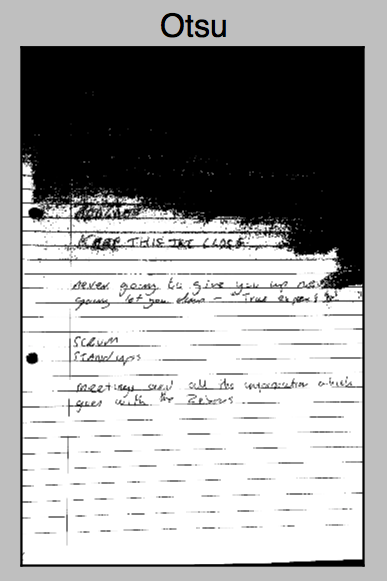
\includegraphics{images/OTSU}
  \label{fig:OTSU}
  \caption{The use of OTSU binarisation technique on an image with a little shadow across the image}
\end{figure}

Figure \ref{fig:OTSU} shows the binarisation technique on an image with the a slight shadow imposed on the image. Clearly it can be seen that it binarises the wrong sections of the image, this would be due to global thresholding.

The basic premise of OTSU is the image's grey-level values are segmented into a series of histograms. OTSU determines the optimial threshold value by ``maximising the discriminant measure''[CITE OTSU PAPTER][CITE OPENCV]. In other words, OTSU attempts to maximise the margin between the histograms. From the maximising of the histograms, pixels can be segmented into their background or foreground pixels. [CITE LAB BROOKS PAGE].

HP, who created Tesseract [CITE], describe OTSU as its underlying pre-processing algorithm when it tries to identify characters. From the iterative spike work with OTSU it is clear to see, just from Figure \ref{fig:OTSU}, how Tesseract would be unable to clearly identify characters from that image.

Overall, OTSU, although it is a very solid binarisation method, it suffers from imposed shadows over images. This would not be the best option to choose when choosing an appropriate binarisation technique.

\subsubsection{Adaptive Threshold} \label{section:threshold}
From the enlighting analysis of OTSU it was realised that using an OTSU thresholding ontop of an OTSU threshold from the Tesseract engine would not be beneficial. Therefore, in the next iteration of the script, an adaptive threshold approach was chosen.

Adaptive threshold will calculate the threshold over a series of smaller segments of the image [CITE]. This reduces the impact of shadows over an image, and does not consider global illumination as the key.

Using the OpenCV library there was two options [CITE OPEN CV]:
\begin{enumerate}
  \item Gaussian adaptive threshold which is the weighted sum of the neighborhood
  \item Mean adaptive threshold, which is the mean of neighborhood.
\end{enumerate}

\begin{figure}[H]
  \centering
  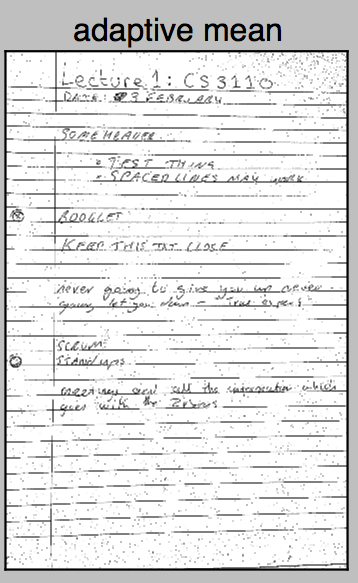
\includegraphics{images/adaptive_mean}
  \caption{Adaptive mean threshold algorithm on a note, showing binarisation but there is still noise in the image.}
  \label{fig:adaptive_mean}
\end{figure}

The mean neighboured takes a block size around the pixel, say 4, and will work out the mean pixel value from that block. The mean value selected will then be selected as the thresholding value, which will determine whether pixels are background or foreground. [CITE] Figure \ref{fig:adaptive_mean} shows a mean adaptive threshold. Due to smoothing issues there is still noise on the image.

The gaussian operation differs from the mean as it uses a gaussian value over the sub-image. Firstly each ``blocksize'' is a value which surround the pixel. A default gaussian weight is then calculated [ADD calculation] based on the blocksize. For every pixel in the block, multiply it by the gaussian, an average weight is then taken and used as a threshold. [CITE LEARN CV][CITE OPEN CV].


\begin{figure}[H]
  \centering
  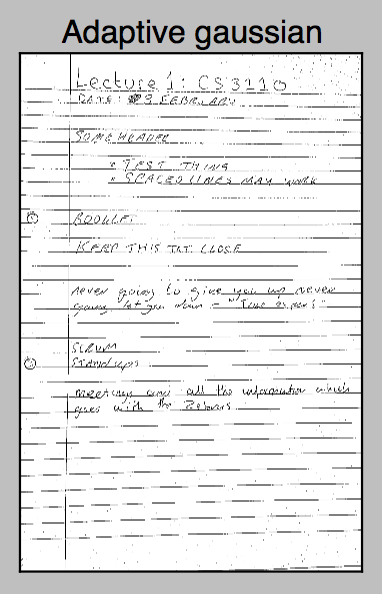
\includegraphics{images/adaptive_gaussian}
  \caption{Adaptive Gaussian used over the image, showing a lot smoother of an image}
  \label{fig:adaptive_gaussian}
\end{figure}

Figure \ref{fig:adaptive_gaussian} shows the adaptive gaussian shows an image which is working it's way to binarisation. It does not have a shadow overlaying the image and the text, lines and little noise have been extracted.

\begin{figure}[H]
  \centering
  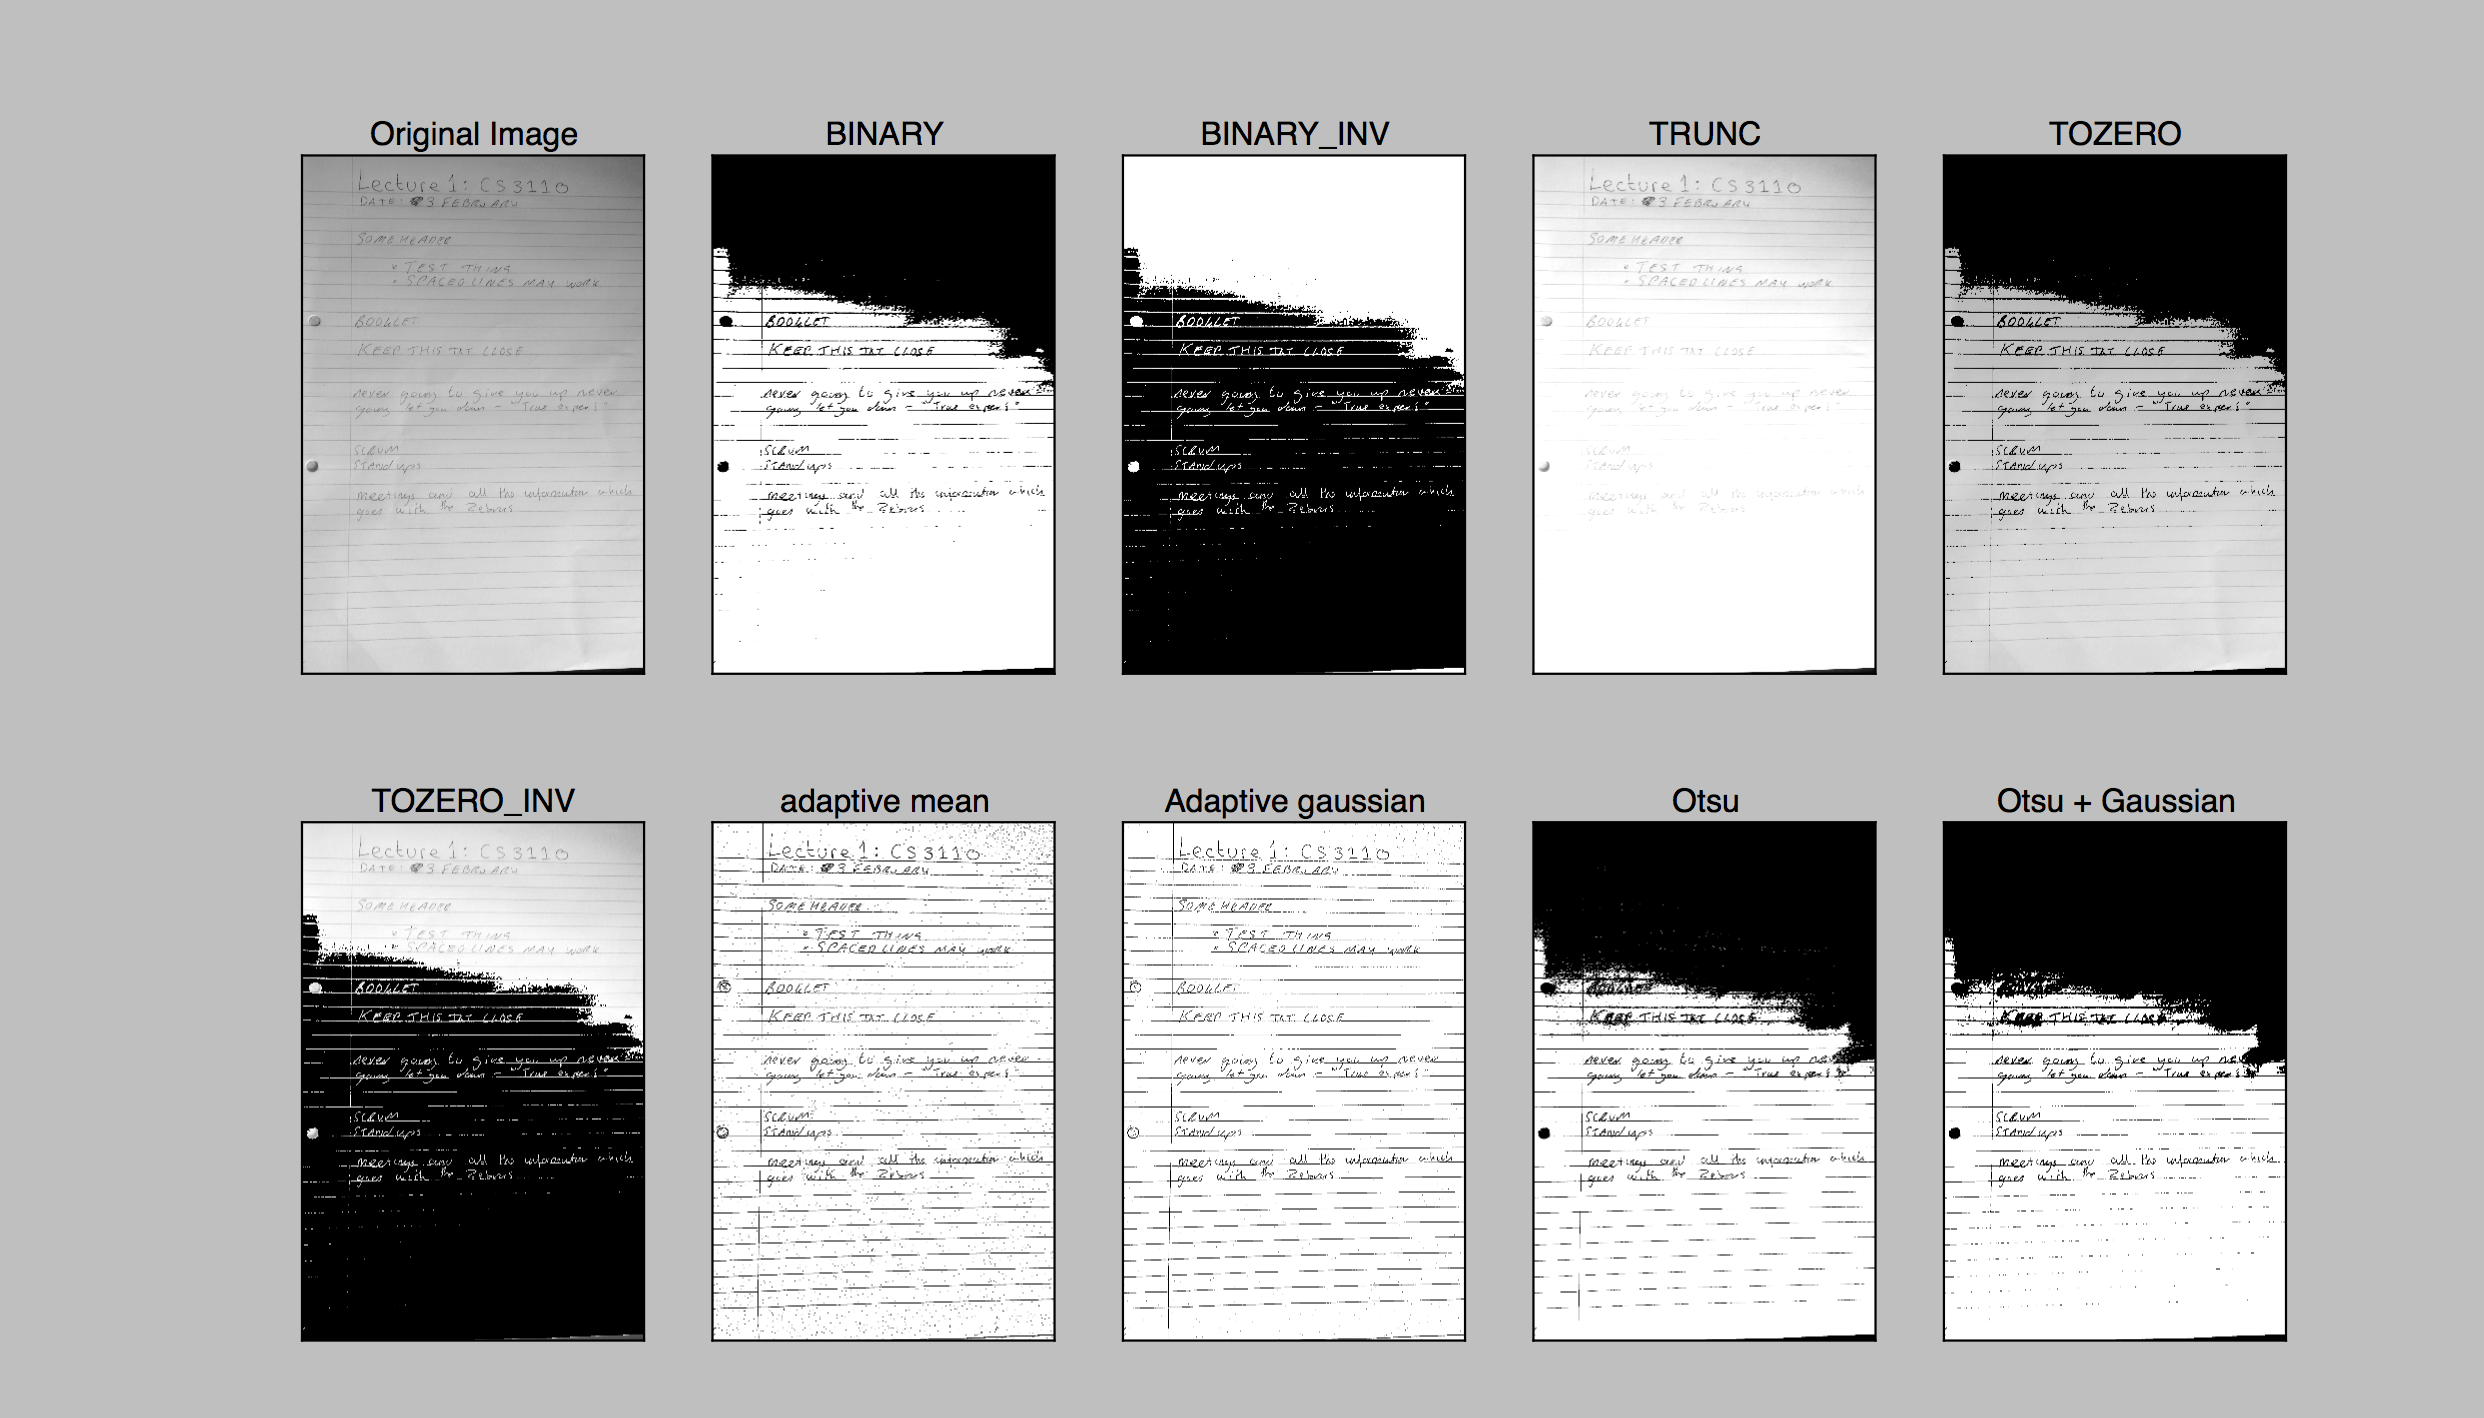
\includegraphics{images/thresholding_options}
  \caption{A variety of thresholding techniques used on the same note, showing adaptive threshold resulting in the best}
  \label{fig:thresholding_options}
\end{figure}

Figure \ref{fig:threshold_options} displays the other types of thresholding options iteratively tried. It was decided that the gaussian adaptive thesholding would be implemented and improved with different morphological operations.

\section{Lined paper}
Intially standard lined paper was used for the notes, but the noise produced from the lines was too much to ensure reliable readings from, Tesseract. Refer to appendix \cite{appendix:image_processing} section \cite{processing:pre-line}.

\subsection{Filtering the blue lines}
Custom lined paper, with equal spacing was constructed to overcome this as discussed in section \ref{}.

Over a few iterations the main aim was to remove the blue lines from the image.
\begin{algorithm}
\caption{Initial removing the blue lines algorithm}
\label{algorithm:threshold1}
\begin{algorithmic}[1]
  \Function(remove\_lines)
    \State $image \gets read\_image\_as\_grayscale()$
    \State $lower\_black \gets np.array([0,0,0])$
    \State $upper\_black \gets np.array([175,20, 95])$
    \State $mask\_black \gets cv2.inRange(erode, lower\_black, upper\_black)$
    \State $mask[np.where(mask\_black == 0)] \gets 255$
  \EndFunction
  \end{algorithmic}
\end{algorithm}

Algorith \ref{algorithm:threshold1} has its obviousy flaws. It attempts to get the values between a grey-black color range. The blue lined tex would obviously have some black content in it, so not all the lines would be removed.

\begin{figure}[H]
  \centering
  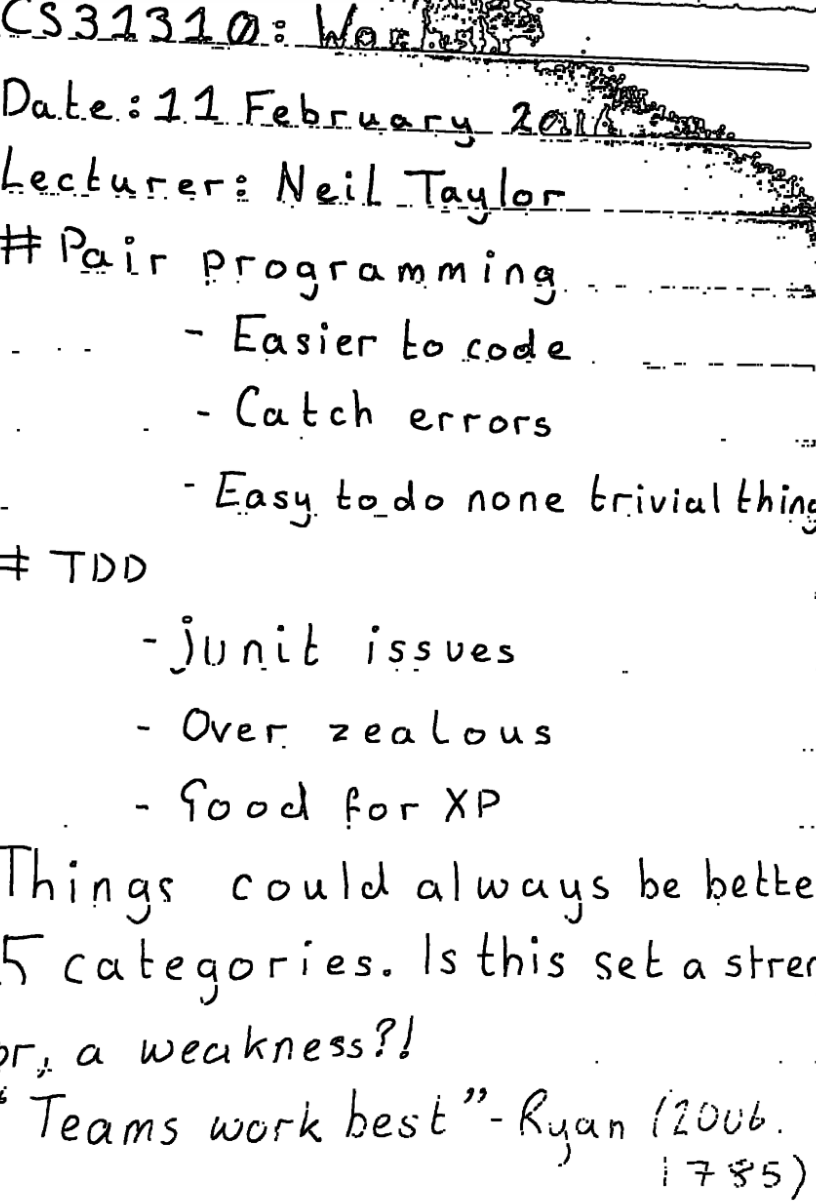
\includegraphics{images/removed_lines_still_noise}
  \caption{An example of the above algorithm. There is still significant amounts of noise in the image.}
  \label{fig:remove_lines_noise}
\end{figure}

After morphological operations such as erroding and dilation, the line noise was no longer being removed and insteadit began to affect the quality of the segmentation, as shown in \ref{fig:remove_lines_noise}. Although these early iterations were not perfect, it was on the write tracks.

\subsection{Only extracting the text}
Due to their being no easy way to identify the lines, but ignore them, then it was decided to just extract the text - bypassing the lines.

OpenCV had a very good example for line extraction [CITE EXAMPLE ON OPEN CV]. After binarising the image, using aforementioned implementation, the horizontal lines wre extracted using OpenCV's structuring element \texttt{Morph\_Rect}[CITE].

Morphologial operations, errosion and dilation, were performed to remove the lines and any additional noise. There was a sereis of blank image masks used an intermediatery step to transfer the text from one image to another. The text was transferred over to the blank mask, but line noise was still being transferred.

Connected components [CITE] via identifying where there were contours on the image was utilised to extract pixels which were connected to one another. Due to different morphological operations, the horizontal lines were not connected completely. As a result the connected components identified all the text in the image - these were then transferred to a new mask.

Finally, errosion was used to remove additional noise and dilation used to fill in and make the characters clearer on the image. Eventually, the binarisation script was complete after a few iterations.

\begin{figure}[H]
  \centering
  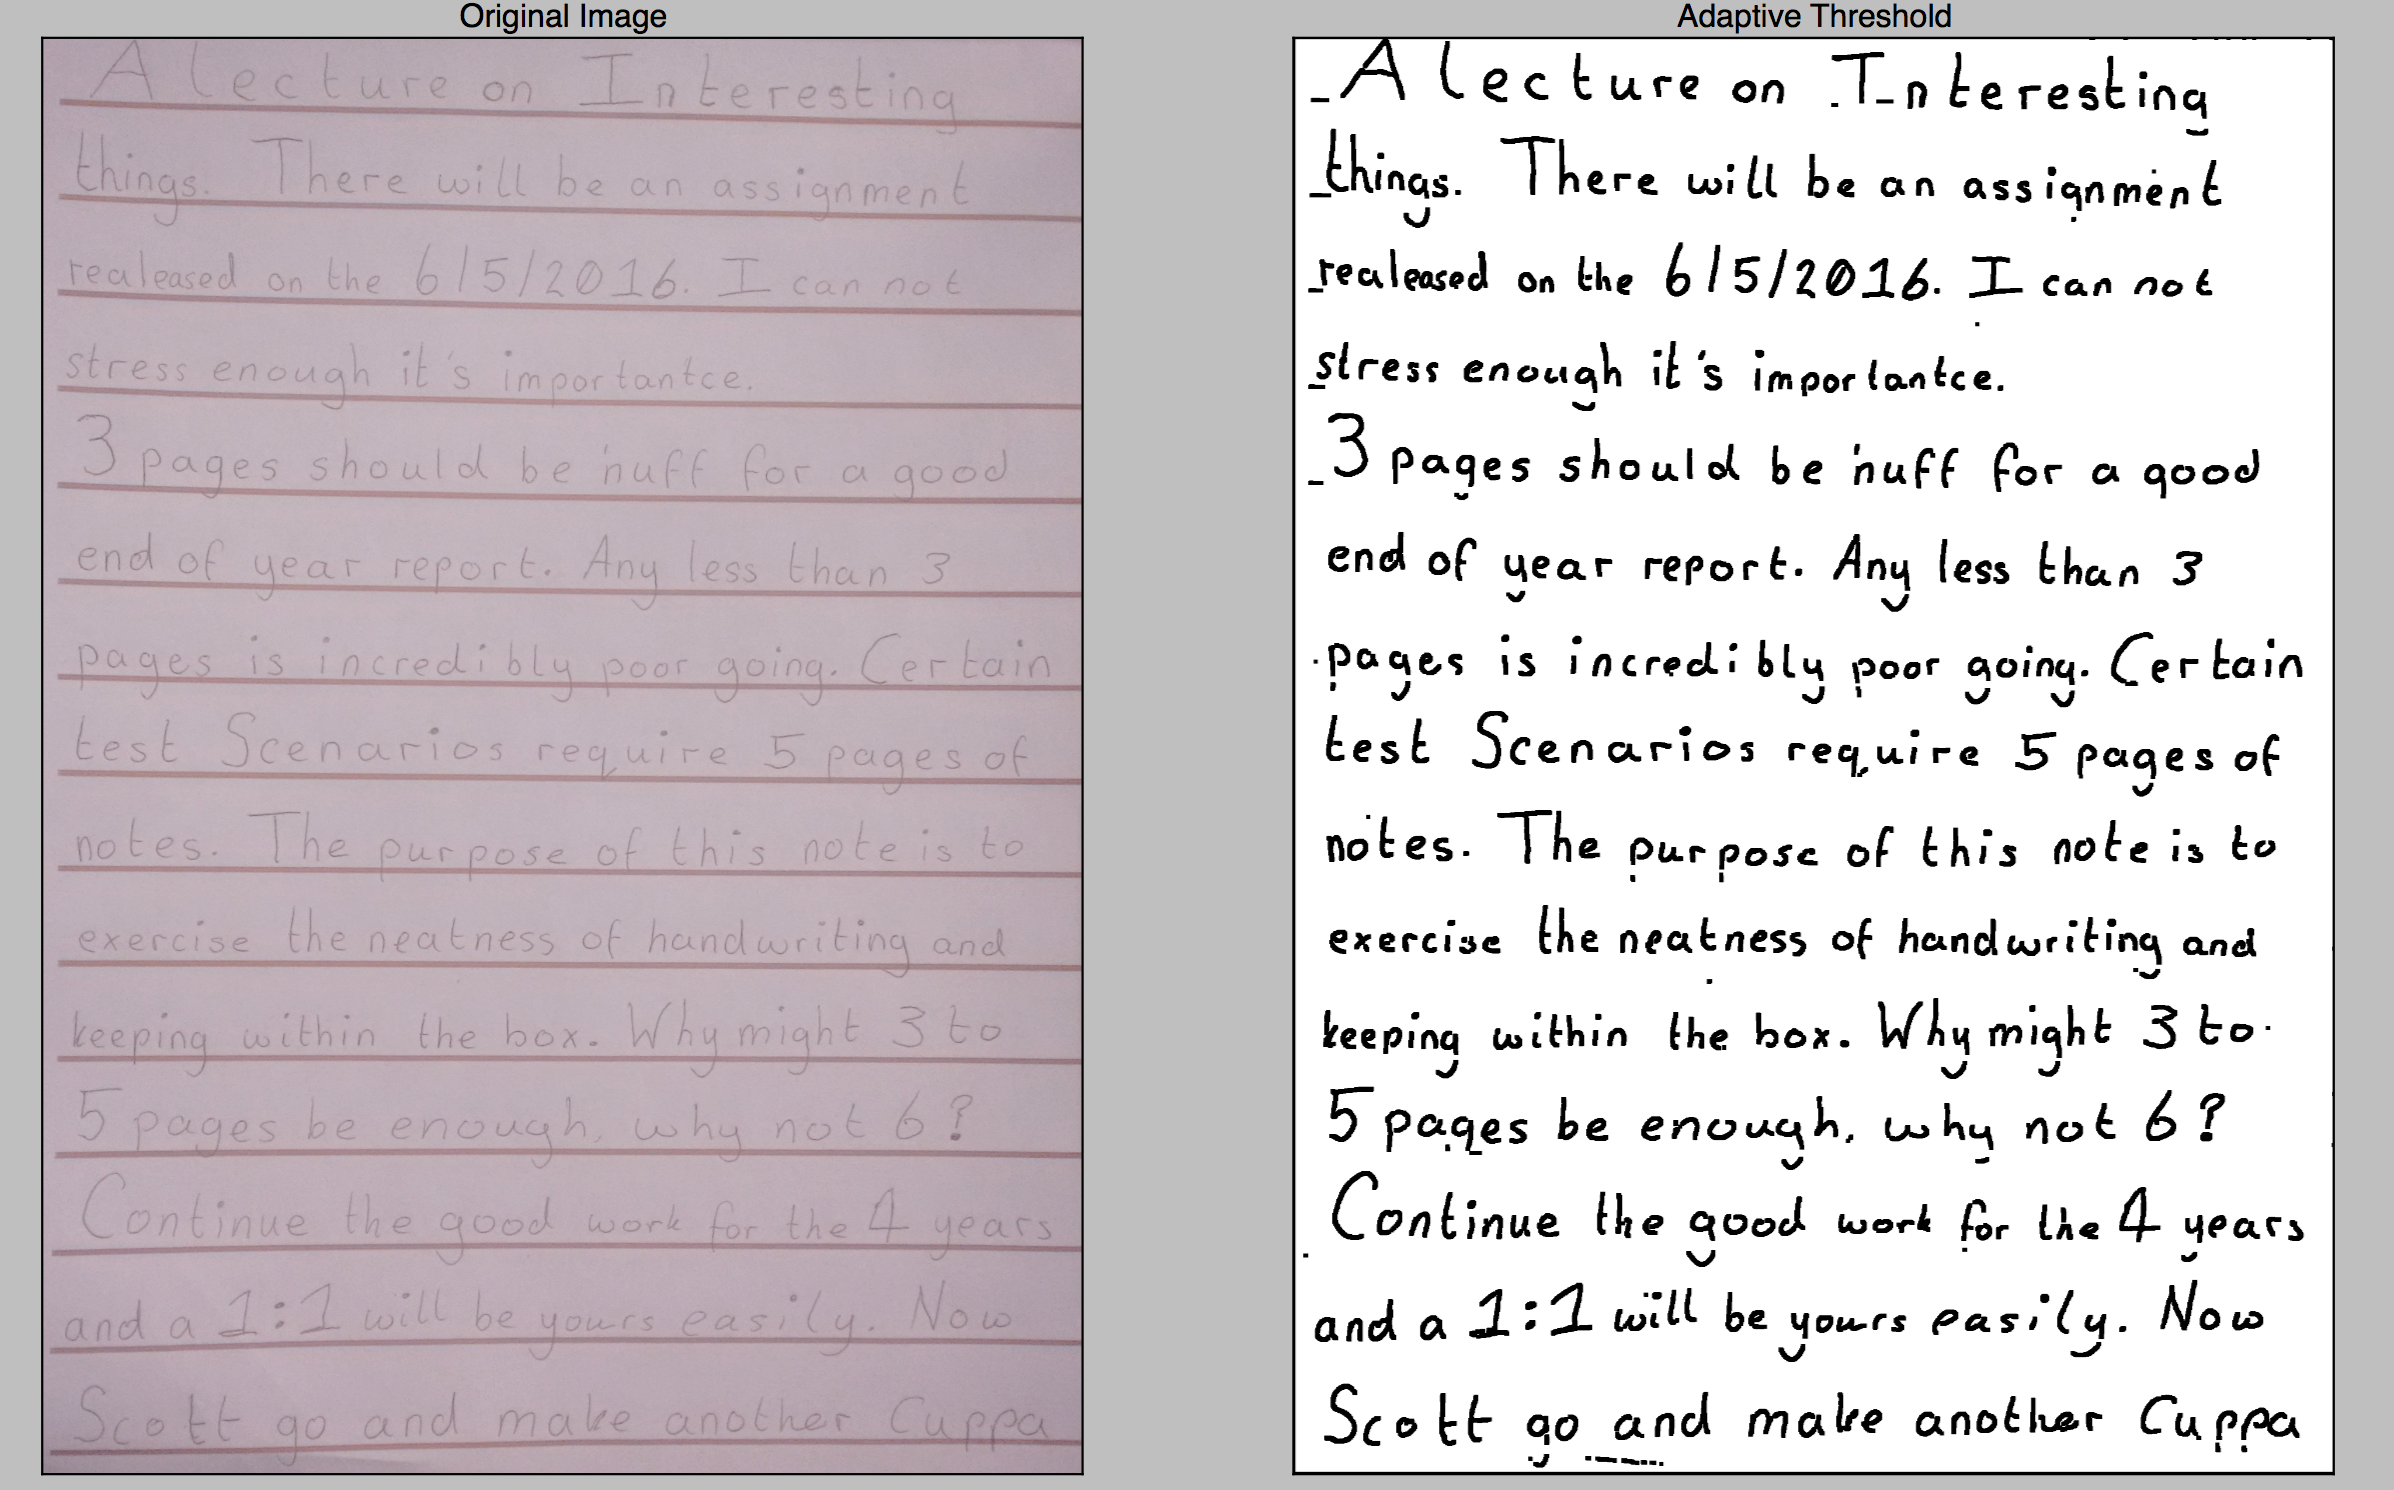
\includegraphics{images/hard_image}
  \caption{A poor quality image has been binarised successfully with little noise.}
  \label{fig:poor_quality}
\end{figure}

As shown in Figure \ref{fig:poor_quality}, the image has been successfully binarised. This shows where adaptive threshold works well - the image is a poor quality image, but it is locally thresheld. Eventually the output of the image is a clean binarisation script, with little noise. There were naturally technical difficulties along the way, and this influenced the implementation decision. Eventually it was agreed the image quality was good enough to stop the binarisation script. Further images of the iterations can be found in Appendix \ref{appendix:image_processing}.

\section{Handwriting Training}
Initially the handwriting training was not yielding a good success rate. After the changes implemented from section \ref{section:threshold} the handwriting training was able to identify more characters successfully.

\subsection{Training process}
Specific files formats were required during the training process with Tesseract; \texttt{<lang>.<font>.exp<number>.tiff} was the layout required for training.

When training on the test images, a selection can be found in Appendix \ref{}, Tesseract outputted a box file which contained all the characters on different lines; each lines consists of coordinates for the box file and the associated character. Initially looking at this file it was hard to identify where it was recognising characters.

\begin{figure}[H]
  \centering
  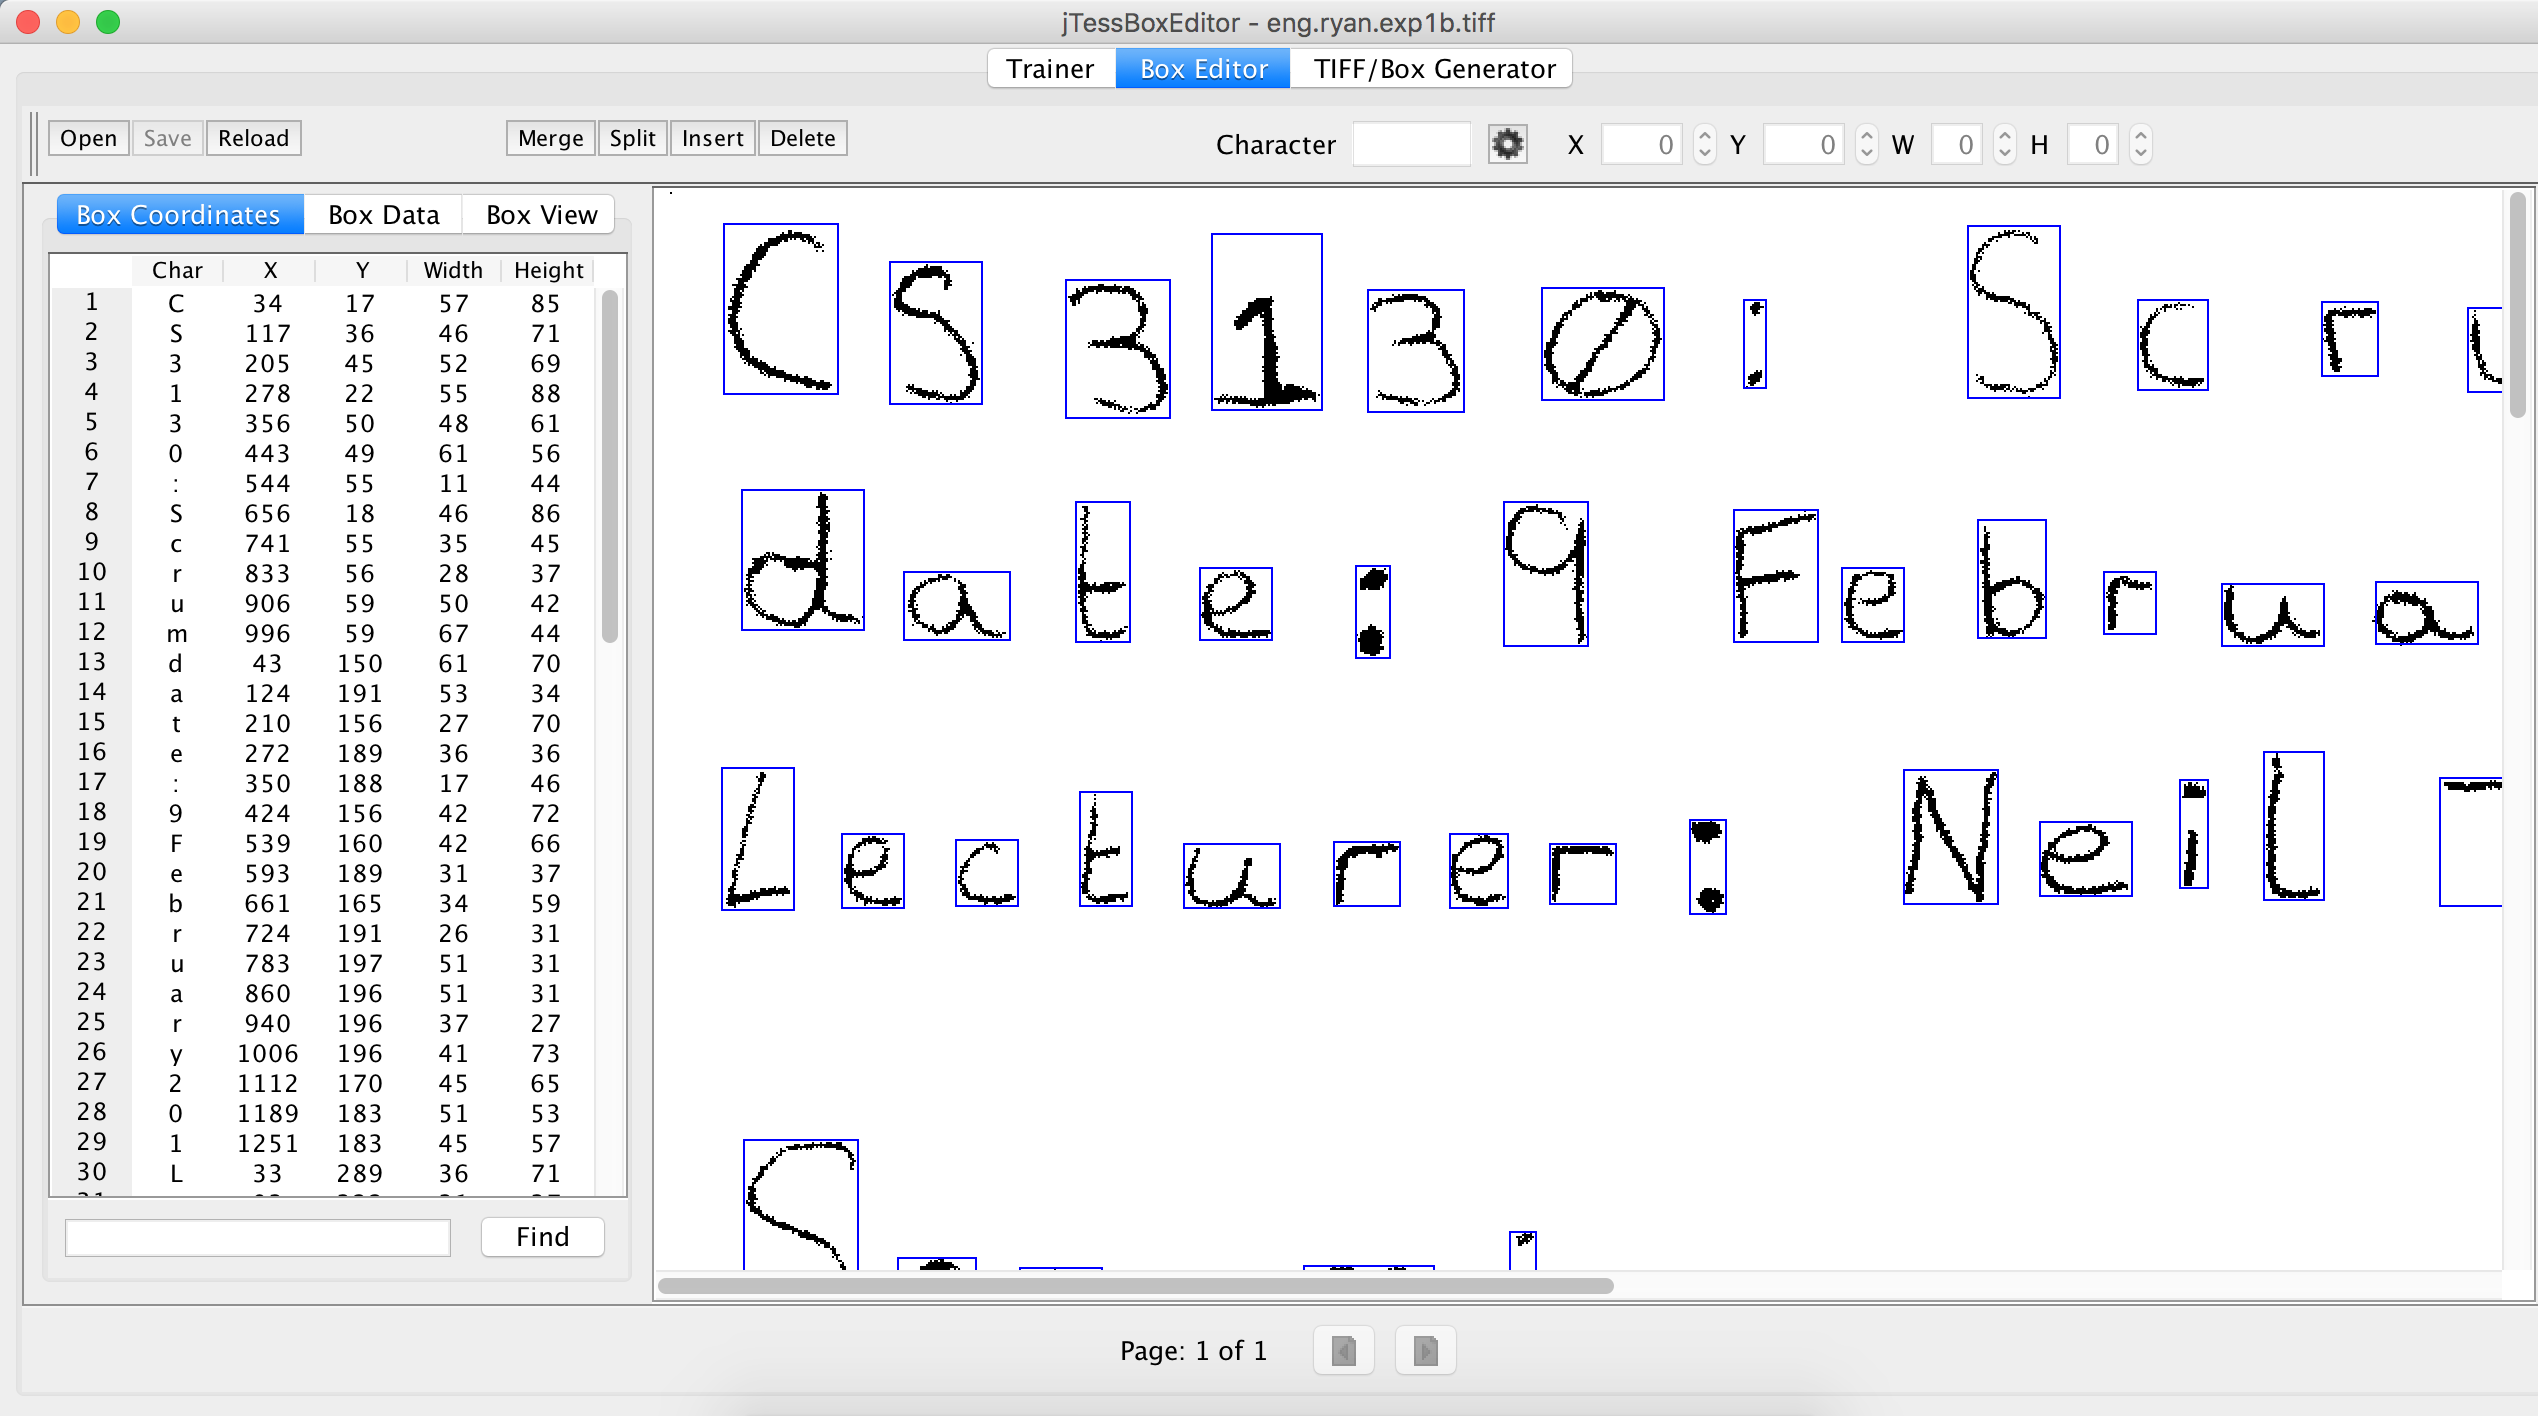
\includegraphics[width=\textwidth]{images/box_editor}
  \label{fig:box_editor}
  \caption{A example of the jTessBoxEditor being used identify characters in the tiff box file.}
\end{figure}

Figure \ref{fig:box_editor} shows the use of the tool jTessBoxEditor [CITE] when re-arranging the boxes and tagging the correct characters.

Issues were identified through the handwriting training section: sometimes characters would not be identified from the image correctly. Often when Tesseract would fail to identify a character correctly it would depict it as ``~''. This would be split and tried to be characterised until Tesseract produced an error saying it failed to identify the characters. After a few iterations of this happening, it was decided that the best option was to remove this line from the box file.

After the tagging of characters had been completed the training process occurred. Refer to appendix \ref{} for more regarding the training process. This process was repeated for each of the 12 training examples.

\section{Web application}

\subsection{OAuth}
Working with the Google OAuth prooved to be quite tricky in some places. Using the Google client library to handle the OAuth2 interactions with the Google API's allowed for a reliable connection and exchanging of tokens.

During the interaction with the Google API's there was a time in which the API client failed and threw a random error. Confused as the service was working the prior day, an issue was made on their GitHub repository [CITE]. This issue miraculously dispearred after a clear of a cache from the API tool.

One issue to consider when dealing with OAuth is handling the refresh tokens. When a user authenticated, the credentials were stored in the user session. In the response from the Google OAuth is a refresh token - this has an expiration date. Prior to realising that the client had a check to see if the expiration token expired, the user would be presented with an error informing them they have an invalid token.

The new implementation redirects them to the logout url and asks them to re-authenticate.

\subsection{Reoccuring events}
Reocurring events were discovered as an issue in the pre-beta user testing. During the design phase when thinking about the calendar, it was forgotten that reocurring events and all-day events could exist.

All-day events do not have the dateTime key response from the Google Calendar API. As a result the code would fail when trying to access the dateTime from the event start date. This resulted in a redesign and re-think of the possible issues which could arise from Google Calendar.

Eventually, the dateTime key was checked and the all day events issue was solved.

However, the reocurring events problem was still existing. When querying for an event, if the event was reocurring then it would group the reocurring events by the first time in which the event was created. This resulted in an image, which was taken on the 12th March 2016 for example, to show events in February - if there was a reocurring event on the 12th March. However, it had an important reoccurence event ID key.

This resulted in a further query being created which would return all the instances that were reocurring. This had to pass in the $event['id']$ to the query to return all these instances; it was filtered down by querying for the start and end date.

When editing a reocurring event, Google calendar performs some unexpected behaviour: instead of silently modifying the event and returning the grouped event, again, it instead returns both the grouped event and the edited event. A succinct solution for this has not been found and has been a slight issue.

\subsection{Tesseract Confidence}
During a meeting with Dr Hannah Dee, it was suggested that some form of confidence score couldbe outputted to the user to show how well Tesseract identifies the text from the image.

The Tesseract command line does not output the confidence of the characters identified; only the C++ library can output the confidence. Due to time constraints, a wrapper for the C++ Tesseract API could not be implemented - so a third party library was chosen, tessocr[CITE].

Tessocr offered the implementation to access the confidence values for the associated words. The algorithm to execute the identification of the characters was quite simple.

Firstly we get all the text lines; Tesseract deals with the lines as a series of text lines. This is then enumerated over and for each line a corresponding list of confidence words is collected from tehe $map_all_words$ API.

Due to this returning a tuple which is an immutable object in Python, modifications on the list could not be made easily. This resulted in the view file checking the tuple content and calculating whether it is above the threshold; 75 for green, 70 for orange and below 65 for red.

\subsection{Displaying calendar events}

\subsection{Parsing Exif data}

\subsection{Editing calendar events}
When adding meta-data to a note, then the date which the user has entered is parsed into a query against the Google Calendar API which would return all the events for that day which they have entered. It would then check the module code entered against the summary field - this would ensure that the events would be found for that given module code.

This potentially displayed the problem of being able to add the note to the wrong event - if there was more than one event with the same module code that day. As a result a further check was conducted to evaluate the date start time and the date which they entered to ensure they matched.

If an event was matched then the event was added to the description field of a given saved note url. One issue which was discovered is that when adding a note it would just replace all the description with the note url and if they were editing it and it no longer existed then it would remove everything from the description. This is naturally bad, as it would mean that a user's description for an event would be overwritten.

This fixed with appending to the end of the description field, for the google calendar. Additionally, a replace was used instead of replacing with an empty string, this preserved the user's content in their description.



\section{Review against the requirements}
